Die Topologie der Infrastruktur beschränkt sich auf das Minimum an Kommunikationsparteien. Dem Thema zufolge sollen ein Mikrocontroller und ein Smartphone sicher Daten austauschen. Um dies zu bewerkstelligen, wird über dem Transport der Daten durch Bluetooth Low Energy (BLE) das Protokoll TLS verwendet (siehe Sektion \ref{sec: infra sicherheit}). Dementsprechend ist, wie in Abb. \ref{fig: infra topologie} zu sehen, neben dem Mikrocontroller und dem Smartphone eine Zertifizierungsstelle notwendig. In welcher Form diese auftritt, ist von der Anwendung abhängig.
\\\\

\begin{figure}[H]
    \centering
    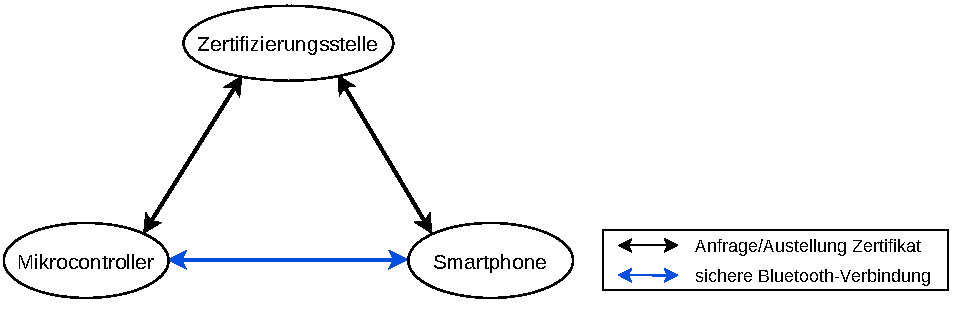
\includegraphics[width=1\textwidth]{graphics/infra_topologie.pdf}
    \caption[Topologie der Infrastruktur]{Topologie der Infrastruktur}
    \label{fig: infra topologie}
\end{figure}

Für einen öffentlich zugänglichen Anwendungsfall sollte die Zertifizierungsstelle dem Mikrocontroller und Smartphone in regelmäßigen Abständen (z.B. jährlich) jeweils ein Zertifikat ausstellen. Mit diesen Zertifikaten und der Kenntnis über das Root"=Zertifikat (das Zertifikat der Zertifizierungsstelle) können Mikrocontroller und Smartphone sich gegenseitig authentifizieren und somit die Grundlage für eine sichere Kommunikation bilden.
\\\\
Für einen einfachen privaten Anwendungsfall, in dem z.B. nur ein einziger Mikrocontroller und ein einziges Smartphone diese Infrastruktur verwenden, würde es genügen, die Schlüsselpaare und Zertifikate auf einer dritten Instanz (z.B. einem Personal Computer) zu generieren und über eine sichere Verbindung (z.B. eine direkte Kabelverbindung) an den Mikrocontroller und das Smartphone zu übertragen.
\\\\
Die Zuweisung der Rollen ist nicht vorgeschrieben. Jedoch wäre es üblich, den Mikrocontroller in Bezug auf BLE als Slave bzw. Peripheral (siehe Sektion \ref{sec: le gap}) und in Bezug auf TLS als Server zu definieren. Folglich würde das Smartphone bzgl. BLE als Master bzw. Central und bzgl. TLS als Client festgelegt werden.